\documentclass[]{book}
\usepackage{lmodern}
\usepackage{amssymb,amsmath}
\usepackage{ifxetex,ifluatex}
\usepackage{fixltx2e} % provides \textsubscript
\ifnum 0\ifxetex 1\fi\ifluatex 1\fi=0 % if pdftex
  \usepackage[T1]{fontenc}
  \usepackage[utf8]{inputenc}
\else % if luatex or xelatex
  \ifxetex
    \usepackage{mathspec}
  \else
    \usepackage{fontspec}
  \fi
  \defaultfontfeatures{Ligatures=TeX,Scale=MatchLowercase}
\fi
% use upquote if available, for straight quotes in verbatim environments
\IfFileExists{upquote.sty}{\usepackage{upquote}}{}
% use microtype if available
\IfFileExists{microtype.sty}{%
\usepackage{microtype}
\UseMicrotypeSet[protrusion]{basicmath} % disable protrusion for tt fonts
}{}
\usepackage{hyperref}
\hypersetup{unicode=true,
            pdftitle={Open tools for writing open interactive textbooks (and more)},
            pdfauthor={Matthew Crump},
            pdfborder={0 0 0},
            breaklinks=true}
\urlstyle{same}  % don't use monospace font for urls
\usepackage{natbib}
\bibliographystyle{apalike}
\usepackage{longtable,booktabs}
\usepackage{graphicx,grffile}
\makeatletter
\def\maxwidth{\ifdim\Gin@nat@width>\linewidth\linewidth\else\Gin@nat@width\fi}
\def\maxheight{\ifdim\Gin@nat@height>\textheight\textheight\else\Gin@nat@height\fi}
\makeatother
% Scale images if necessary, so that they will not overflow the page
% margins by default, and it is still possible to overwrite the defaults
% using explicit options in \includegraphics[width, height, ...]{}
\setkeys{Gin}{width=\maxwidth,height=\maxheight,keepaspectratio}
\IfFileExists{parskip.sty}{%
\usepackage{parskip}
}{% else
\setlength{\parindent}{0pt}
\setlength{\parskip}{6pt plus 2pt minus 1pt}
}
\setlength{\emergencystretch}{3em}  % prevent overfull lines
\providecommand{\tightlist}{%
  \setlength{\itemsep}{0pt}\setlength{\parskip}{0pt}}
\setcounter{secnumdepth}{5}
% Redefines (sub)paragraphs to behave more like sections
\ifx\paragraph\undefined\else
\let\oldparagraph\paragraph
\renewcommand{\paragraph}[1]{\oldparagraph{#1}\mbox{}}
\fi
\ifx\subparagraph\undefined\else
\let\oldsubparagraph\subparagraph
\renewcommand{\subparagraph}[1]{\oldsubparagraph{#1}\mbox{}}
\fi

%%% Use protect on footnotes to avoid problems with footnotes in titles
\let\rmarkdownfootnote\footnote%
\def\footnote{\protect\rmarkdownfootnote}

%%% Change title format to be more compact
\usepackage{titling}

% Create subtitle command for use in maketitle
\providecommand{\subtitle}[1]{
  \posttitle{
    \begin{center}\large#1\end{center}
    }
}

\setlength{\droptitle}{-2em}

  \title{Open tools for writing open interactive textbooks (and more)}
    \pretitle{\vspace{\droptitle}\centering\huge}
  \posttitle{\par}
    \author{Matthew Crump}
    \preauthor{\centering\large\emph}
  \postauthor{\par}
      \predate{\centering\large\emph}
  \postdate{\par}
    \date{2018: Last compiled 2019-06-22}

\usepackage{booktabs}
\usepackage{amsthm}
\makeatletter
\def\thm@space@setup{%
  \thm@preskip=8pt plus 2pt minus 4pt
  \thm@postskip=\thm@preskip
}
\makeatother

\begin{document}
\maketitle

{
\setcounter{tocdepth}{1}
\tableofcontents
}
\hypertarget{preface}{%
\chapter*{Preface}\label{preface}}
\addcontentsline{toc}{chapter}{Preface}

\begin{center}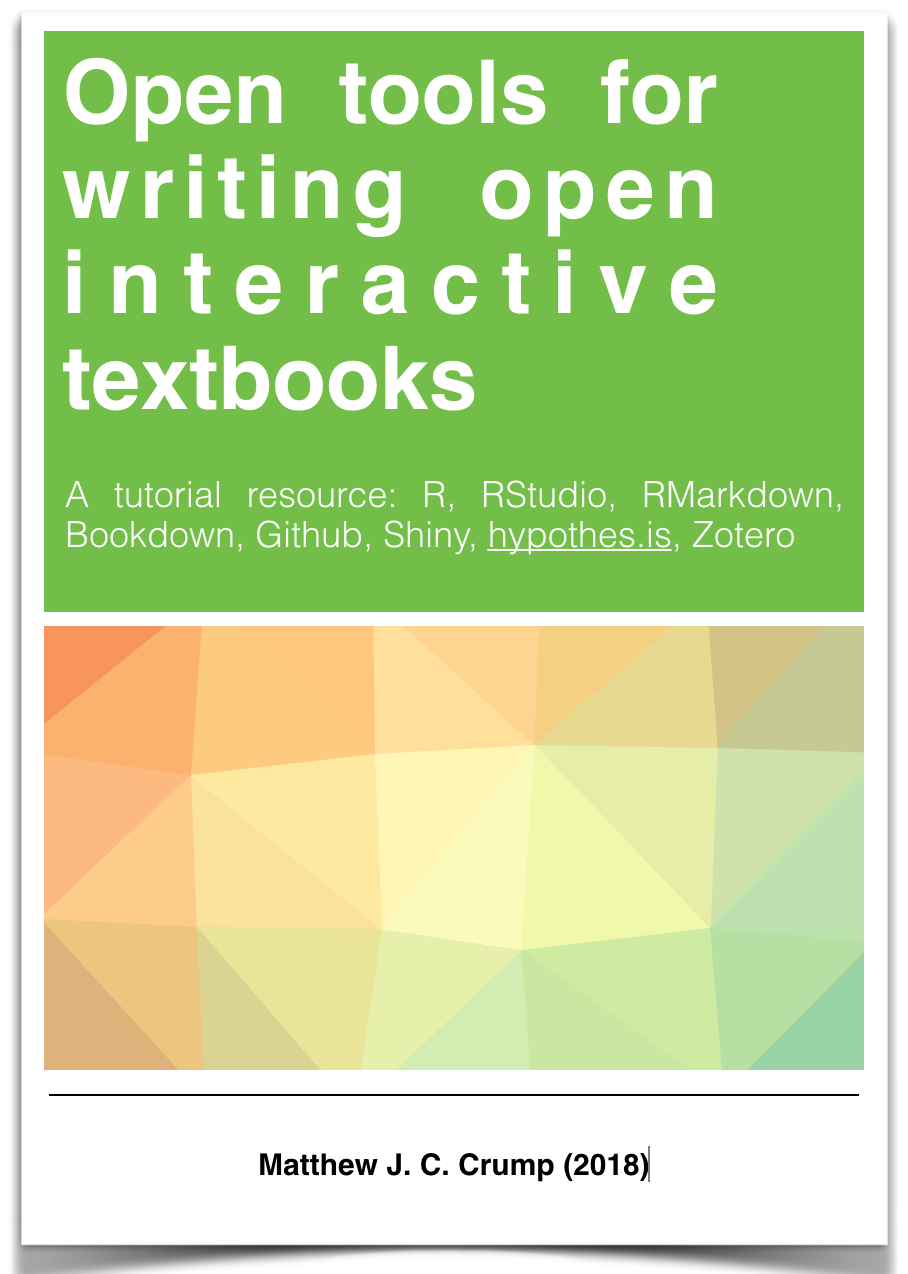
\includegraphics{OER} \end{center}

Crump, Matthew J. C. (2018). Open tools for writing open interactive textbooks (and more). \url{https://crumplab.github.io/programmingforpsych/}

This is a tutorial and set of working examples for creating web-based textbooks using a collection of open-source tools.

This web-book is itself a working example. All of the source code needed to compile this book yourself is included in the \href{https://github.com/CrumpLab/OER_bookdown}{github repository for this book}. So, you could download the repository, and by following the instructions laid out across the chapters, replace this text with your own, and then compile your book as a web-page, .pdf or epub.

Feel free to contribute to this tutorial by submitting pull requests to this repository.

\textbf{License CC BY-SA 4.0 license}

The book is released under a creative commons \href{https://creativecommons.org/licenses/by-sa/4.0/}{CC BY-SA 4.0} license. This means that this book can be reused, remixed, retained, revised and redistributed (including commercially) as long as appropriate credit is given to the authors. If you remix, or modify the original version of this open textbook, you must redistribute all versions of this open textbook under the same license - CC BY-SA 4.0.

\hypertarget{Quadratics}{%
\chapter{Quadratic Functions and Factoring}\label{Quadratics}}

\hypertarget{review-of-functions}{%
\section{Review of Functions}\label{review-of-functions}}

\hypertarget{what-is-a-function}{%
\subsection{What is a Function}\label{what-is-a-function}}

\hypertarget{parent-functions}{%
\subsection{Parent Functions}\label{parent-functions}}

\hypertarget{constant}{%
\subsubsection{Constant}\label{constant}}

\hypertarget{linear}{%
\subsubsection{Linear}\label{linear}}

\hypertarget{absolute-vavlue}{%
\subsubsection{Absolute Vavlue}\label{absolute-vavlue}}

\hypertarget{function-operations}{%
\subsection{Function Operations}\label{function-operations}}

\hypertarget{arithmetic-operations}{%
\subsubsection{Arithmetic Operations}\label{arithmetic-operations}}

\hypertarget{composition}{%
\subsubsection{Composition}\label{composition}}

\hypertarget{inverse-functions}{%
\subsection{Inverse Functions}\label{inverse-functions}}

\hypertarget{finding-inverse-functions}{%
\subsubsection{Finding Inverse Functions}\label{finding-inverse-functions}}

\hypertarget{qudaratic-functions-in-vertex-form}{%
\section{Qudaratic Functions in Vertex Form}\label{qudaratic-functions-in-vertex-form}}

\hypertarget{graphing}{%
\subsection{Graphing}\label{graphing}}

\hypertarget{solving}{%
\subsection{Solving}\label{solving}}

\hypertarget{quadratic-functions-in-standard-form}{%
\section{Quadratic Functions in Standard Form}\label{quadratic-functions-in-standard-form}}

\hypertarget{graphing-1}{%
\subsection{Graphing}\label{graphing-1}}

\hypertarget{factoring}{%
\subsection{Factoring}\label{factoring}}

\hypertarget{factoring-x2bxc}{%
\subsubsection{\texorpdfstring{Factoring \(x^2+bx+c\)}{Factoring x\^{}2+bx+c}}\label{factoring-x2bxc}}

\hypertarget{factoring-ax2bxc}{%
\subsubsection{\texorpdfstring{Factoring \(ax^2+bx+c\)}{Factoring ax\^{}2+bx+c}}\label{factoring-ax2bxc}}

\hypertarget{solving-1}{%
\subsection{Solving}\label{solving-1}}

\hypertarget{quadratic-functions-in-intecept-form}{%
\section{Quadratic Functions in Intecept Form}\label{quadratic-functions-in-intecept-form}}

\hypertarget{graphing-2}{%
\subsection{Graphing}\label{graphing-2}}

\hypertarget{other-methods}{%
\section{Other Methods}\label{other-methods}}

\hypertarget{completing-the-square}{%
\subsection{Completing the Square}\label{completing-the-square}}

\hypertarget{quadratic-formula}{%
\subsection{Quadratic Formula}\label{quadratic-formula}}

\hypertarget{quadratic-modeling}{%
\section{Quadratic Modeling}\label{quadratic-modeling}}

\hypertarget{using-vertex-and-one-point}{%
\subsection{Using Vertex and One Point}\label{using-vertex-and-one-point}}

\hypertarget{using-an-intercept-and-one-point}{%
\subsection{Using an Intercept and One Point}\label{using-an-intercept-and-one-point}}

\hypertarget{using-three-points}{%
\subsection{Using Three Points}\label{using-three-points}}

\hypertarget{technological-tools}{%
\subsection{Technological Tools}\label{technological-tools}}

\hypertarget{review-exercises}{%
\section{Review Exercises}\label{review-exercises}}

\hypertarget{Polynomials}{%
\chapter{Polynomials and Polynomial Functions}\label{Polynomials}}

\hypertarget{review-properties-of-exponents}{%
\section{Review: Properties of Exponents}\label{review-properties-of-exponents}}

\hypertarget{basics-polynomial-functions}{%
\section{Basics Polynomial Functions}\label{basics-polynomial-functions}}

\hypertarget{fundamentals}{%
\subsection{Fundamentals}\label{fundamentals}}

\hypertarget{polynomial-operations}{%
\subsection{Polynomial Operations}\label{polynomial-operations}}

\hypertarget{end-behavior}{%
\subsection{End Behavior}\label{end-behavior}}

\hypertarget{zeros}{%
\subsection{Zeros}\label{zeros}}

\hypertarget{graphs-of-polynomial-functions}{%
\section{Graphs of Polynomial Functions}\label{graphs-of-polynomial-functions}}

\hypertarget{intercept-form}{%
\subsection{Intercept Form}\label{intercept-form}}

\hypertarget{equations-of-polynomial-functions-from-graph}{%
\subsection{Equations of Polynomial Functions from Graph}\label{equations-of-polynomial-functions-from-graph}}

\hypertarget{factor-and-solve-polynomial-equations}{%
\section{Factor and Solve Polynomial Equations}\label{factor-and-solve-polynomial-equations}}

\hypertarget{special-patterns}{%
\subsection{Special Patterns}\label{special-patterns}}

\hypertarget{factoring-tools}{%
\subsection{Factoring Tools}\label{factoring-tools}}

\hypertarget{remainder-and-factor-theorem}{%
\subsubsection{Remainder and Factor Theorem}\label{remainder-and-factor-theorem}}

\hypertarget{synthetic-division-and-substitution}{%
\subsubsection{Synthetic Division and Substitution}\label{synthetic-division-and-substitution}}

\hypertarget{rational-root-theorem}{%
\subsubsection{Rational Root Theorem}\label{rational-root-theorem}}

\hypertarget{descartes-rule-of-signs}{%
\subsubsection{Descartes Rule of Signs}\label{descartes-rule-of-signs}}

\hypertarget{fundamental-theorem-of-algebra}{%
\subsubsection{Fundamental Theorem of Algebra}\label{fundamental-theorem-of-algebra}}

\hypertarget{find-rational-zeros}{%
\subsection{Find Rational Zeros}\label{find-rational-zeros}}

\hypertarget{find-real-zeros}{%
\subsection{Find Real Zeros}\label{find-real-zeros}}

\hypertarget{analyze-grapsh-of-polynomial-functions}{%
\section{Analyze Grapsh of Polynomial Functions}\label{analyze-grapsh-of-polynomial-functions}}

\hypertarget{writing-least-degree-polynomial-function-from-graph}{%
\subsection{Writing Least Degree Polynomial Function from Graph}\label{writing-least-degree-polynomial-function-from-graph}}

\hypertarget{Rational}{%
\chapter{Rational Expressions, Equations, and Functions}\label{Rational}}

\hypertarget{reciprocal-function-fxfrac1x}{%
\section{\texorpdfstring{Reciprocal Function \(f(x)=\frac{1}{x}\)}{Reciprocal Function f(x)=\textbackslash{}frac\{1\}\{x\}}}\label{reciprocal-function-fxfrac1x}}

\hypertarget{graph-of-reciprocal-function}{%
\subsection{Graph of Reciprocal Function}\label{graph-of-reciprocal-function}}

\hypertarget{transformation-of-graphs}{%
\subsection{Transformation of Graphs}\label{transformation-of-graphs}}

\hypertarget{change-fxfracxaxb-to-fxfracax-hk}{%
\subsection{\texorpdfstring{Change \(f(x)=\frac{x+a}{x+b}\) to \(f(x)=\frac{a}{x-h}+k\)}{Change f(x)=\textbackslash{}frac\{x+a\}\{x+b\} to f(x)=\textbackslash{}frac\{a\}\{x-h\}+k}}\label{change-fxfracxaxb-to-fxfracax-hk}}

\hypertarget{model-inverse-and-joint-variation}{%
\subsection{Model Inverse and Joint Variation}\label{model-inverse-and-joint-variation}}

\hypertarget{rational-expressions}{%
\section{Rational Expressions}\label{rational-expressions}}

\hypertarget{multiply-and-divide-rational-expressions}{%
\subsection{Multiply and Divide Rational Expressions}\label{multiply-and-divide-rational-expressions}}

\hypertarget{add-and-subtract-rational-expressions}{%
\subsection{Add and Subtract Rational Expressions}\label{add-and-subtract-rational-expressions}}

\hypertarget{graph-rational-functions}{%
\section{Graph Rational Functions}\label{graph-rational-functions}}

\hypertarget{rules-for-graphing-rational-functions}{%
\subsection{Rules for Graphing Rational Functions}\label{rules-for-graphing-rational-functions}}

\hypertarget{solve-rational-equations}{%
\section{Solve Rational Equations}\label{solve-rational-equations}}

\hypertarget{writing-rational-equations-from-graphs}{%
\section{Writing Rational Equations from Graphs}\label{writing-rational-equations-from-graphs}}

\hypertarget{partial-fraction-decomposition}{%
\section{Partial Fraction Decomposition}\label{partial-fraction-decomposition}}

\hypertarget{rational-exponents-and-radical-functions}{%
\chapter{Rational Exponents and Radical Functions}\label{rational-exponents-and-radical-functions}}

\hypertarget{evaluate-nth-roots-and-use-rational-exponents}{%
\section{Evaluate nth Roots and Use Rational Exponents}\label{evaluate-nth-roots-and-use-rational-exponents}}

\hypertarget{apply-properties-of-rational-exponents}{%
\section{Apply Properties of Rational Exponents}\label{apply-properties-of-rational-exponents}}

\hypertarget{function-operations-and-inverses-revisited}{%
\section{Function Operations and Inverses Revisited}\label{function-operations-and-inverses-revisited}}

\hypertarget{graph-square-root-and-cube-root-functions}{%
\section{Graph Square Root and Cube Root Functions}\label{graph-square-root-and-cube-root-functions}}

\hypertarget{solve-radical-equations}{%
\section{Solve Radical Equations}\label{solve-radical-equations}}

\hypertarget{exponential-and-logarithmic-functions}{%
\chapter{Exponential and Logarithmic Functions}\label{exponential-and-logarithmic-functions}}

\hypertarget{exponential-functions}{%
\section{Exponential Functions}\label{exponential-functions}}

\hypertarget{standard-form}{%
\subsection{Standard Form}\label{standard-form}}

\hypertarget{growth}{%
\subsubsection{Growth}\label{growth}}

\hypertarget{decay}{%
\subsubsection{Decay}\label{decay}}

\hypertarget{graphs}{%
\subsection{Graphs}\label{graphs}}

\hypertarget{growth-1}{%
\subsubsection{Growth}\label{growth-1}}

\hypertarget{decay-1}{%
\subsubsection{Decay}\label{decay-1}}

\hypertarget{the-exponential-function}{%
\subsection{The Exponential Function}\label{the-exponential-function}}

\hypertarget{logarithmic-functions}{%
\section{Logarithmic Functions}\label{logarithmic-functions}}

\hypertarget{definition-of-a-logarithm}{%
\subsection{Definition of a Logarithm}\label{definition-of-a-logarithm}}

\hypertarget{properties-of-logarithms}{%
\subsection{Properties of Logarithms}\label{properties-of-logarithms}}

\hypertarget{graphs-of-logarithmic-functions}{%
\subsection{Graphs of Logarithmic Functions}\label{graphs-of-logarithmic-functions}}

\hypertarget{solve-exponential-and-logarithmic-equations}{%
\section{Solve Exponential and Logarithmic Equations}\label{solve-exponential-and-logarithmic-equations}}

\hypertarget{write-and-apply-exponential-and-power-functions}{%
\section{Write and Apply Exponential and Power Functions}\label{write-and-apply-exponential-and-power-functions}}

\hypertarget{trigonometry}{%
\chapter{Trigonometry}\label{trigonometry}}

\hypertarget{angle-measurement}{%
\section{Angle Measurement}\label{angle-measurement}}

\hypertarget{right-triangle-trigonometry}{%
\section{Right Triangle Trigonometry}\label{right-triangle-trigonometry}}

\hypertarget{trigonometry-of-any-angle}{%
\section{Trigonometry of Any Angle}\label{trigonometry-of-any-angle}}

\hypertarget{unit-circle-trigonometry}{%
\section{Unit Circle Trigonometry}\label{unit-circle-trigonometry}}

\hypertarget{evaluate-inverse-trigonometric-functions}{%
\section{Evaluate Inverse Trigonometric Functions}\label{evaluate-inverse-trigonometric-functions}}

\hypertarget{law-of-sines}{%
\section{Law of Sines}\label{law-of-sines}}

\hypertarget{law-of-cosines}{%
\section{Law of Cosines}\label{law-of-cosines}}

\hypertarget{trigonometric-graphs}{%
\section{Trigonometric Graphs}\label{trigonometric-graphs}}

\hypertarget{write-trigonometric-models}{%
\section{Write Trigonometric Models}\label{write-trigonometric-models}}

\hypertarget{trigonometric-identities}{%
\section{Trigonometric Identities}\label{trigonometric-identities}}

\hypertarget{solve-trigonometric-equations}{%
\section{Solve Trigonometric Equations}\label{solve-trigonometric-equations}}

\hypertarget{data-analysis-and-statistics}{%
\chapter{Data Analysis and Statistics}\label{data-analysis-and-statistics}}

\hypertarget{combinations-and-the-binomial-theorem}{%
\section{Combinations and the Binomial Theorem}\label{combinations-and-the-binomial-theorem}}

\hypertarget{binomial-distributions}{%
\section{Binomial Distributions}\label{binomial-distributions}}

\hypertarget{normal-distributions}{%
\section{Normal Distributions}\label{normal-distributions}}

\hypertarget{sequences-and-series}{%
\chapter{Sequences and Series}\label{sequences-and-series}}

\hypertarget{define-and-use-sequences-and-series}{%
\section{Define and Use Sequences and Series}\label{define-and-use-sequences-and-series}}

\hypertarget{arithmetic-sequences-and-series}{%
\section{Arithmetic Sequences and Series}\label{arithmetic-sequences-and-series}}

\hypertarget{geometric-sequences-and-series}{%
\section{Geometric Sequences and Series}\label{geometric-sequences-and-series}}

\hypertarget{sums-of-infinite-geometric-series}{%
\section{Sums of Infinite Geometric Series}\label{sums-of-infinite-geometric-series}}

\hypertarget{recursive-rules}{%
\section{Recursive Rules}\label{recursive-rules}}

\hypertarget{quadratic-relations-and-conic-sections}{%
\chapter{Quadratic Relations and Conic Sections}\label{quadratic-relations-and-conic-sections}}

\hypertarget{apply-distance-and-midpoint-formukas}{%
\section{Apply Distance and Midpoint Formukas}\label{apply-distance-and-midpoint-formukas}}

\hypertarget{parabolas}{%
\section{Parabolas}\label{parabolas}}

\hypertarget{circles}{%
\section{Circles}\label{circles}}

\hypertarget{ellispes}{%
\section{Ellispes}\label{ellispes}}

\hypertarget{hyperbolas}{%
\section{Hyperbolas}\label{hyperbolas}}

\hypertarget{translate-and-classify-conic-sections}{%
\section{Translate and Classify Conic Sections}\label{translate-and-classify-conic-sections}}

\hypertarget{solve-quadratic-systems}{%
\section{Solve Quadratic Systems}\label{solve-quadratic-systems}}

\bibliography{book.bib,packages.bib}


\end{document}
